\documentclass[a4paper,12pt,titlepage]{report}

\usepackage[utf8]{inputenc}
\usepackage[T1]{fontenc}
\usepackage[french]{babel}
\usepackage{mathtools,amssymb,amsthm}
\usepackage[top=20mm, bottom=25mm, left=15mm, right=15mm]{geometry}
\usepackage{hyperref}
\usepackage{xcolor}

\newcommand{\octave}{\textit{Octave }}

\setcounter{secnumdepth}{3}
\renewcommand{\thesection}{\arabic{section}.}
\renewcommand{\thesubsection}{\arabic{section}.\arabic{subsection}}
%\titleformat{\subsubsection}[runin]{\normalfont\bfseries}{\thesubsubsection}{0em}{}

\title{Second Rapport d'Avancement Projet Signal\\Reconnaissance Optique de Caractères}
\author{Tristan DRUSSEL - Florian POUTHIER \\ \\ Génie Électrique - 4ème année\\ INSA Strasbourg}
\date{Année scolaire 2019-2020}

\begin{document}
	\begin{titlepage}
		\maketitle
	\end{titlepage}
	\tableofcontents
	\newpage
	\section{Introduction}
		Dans le cadre du cours de signal dispensé au semestre 8 de la formation en Génie Électrique, nous devons réaliser un projet utilisant les compétences et connaissances acquises dans le cours mais aussi les approfondir dans le domaine qui concerne notre sujet.
		Notre sujet est la \textit{Reconnaissance Optique de Caractères (ROC)}. Avec les méthodes et les outils de traitement du signal, nous allons pouvoir comparer des caractères et ainsi transformer une photo en un fichier texte numérique. Vous pouvez retrouver l'intégralité de nos codes sur notre dépôt \href{https://github.com/tristanplouz/ProjetSignal}{github ici}.
		\subsection{Une image, un signal?}	
		La première des choses à faire est de définir l'image. Une image en informatique est un tableau où l'image est découpée en petits carrés. Chaque case du tableau correspond à un petit carré de l'image et le contenu du tableau est la quantité de rouge, de vert et de bleu de chaque découpage. Plus il y a de découpage plus l'image est précise.
		Afin que l'image devienne un objet mathématique nous pouvons la transformer en une matrice. Le tableau défini précédemment peut donc devenir la matrice suivante:
		\begin{equation}
		\begin{bmatrix} 
		\begin{pmatrix} r_{1,1} \\ g_{1,1}\\ b_{1,1} \end{pmatrix} &\begin{pmatrix} r_{2,1} \\ g_{2,1}\\ b_{2,1} \end{pmatrix}&\begin{pmatrix} r_{3,1} \\ g_{3,1}\\ b_{3,1} \end{pmatrix} 
		\\ \begin{pmatrix} r_{1,2} \\ g_{1,2}\\ b_{1,2} \end{pmatrix} & \begin{pmatrix} r_{2,2} \\ g_{2,2}\\ b_{2,2} \end{pmatrix}&\begin{pmatrix} r_{3,2} \\ g_{3,2}\\ b_{3,2} \end{pmatrix}
		\\ \begin{pmatrix} r_{1,3} \\ g_{1,3}\\ b_{1,3} \end{pmatrix} & \begin{pmatrix} r_{2,3} \\ g_{2,3}\\ b_{2,3} \end{pmatrix}&\begin{pmatrix} r_{3,3} \\ g_{3,3}\\ b_{3,3} \end{pmatrix} 
		\end{bmatrix}
		\end{equation}
		Cette matrice de $ M_{m,n}([0,255]^3)$ permet donc de représenter n'importe quelle image et a autant de coefficients que l'image est décomposée en petites cases.
		Cette écriture est pratique, en effet nous avons accès à chaque proportion de couleur de chaque découpage. En revanche travailler avec des matrices de vecteurs n'est pas chose simple. Nous allons donc transformer cette matrice en une matrice d'éléments de $I=[0,255]$. Pour cela nous avons plusieurs solutions, nous pouvons créer une image en nuance de rouge, on ne prend que la première composante du vecteur de chaque case, en nuance de vert, en prenant la seconde, en nuance de bleu en prenant la dernière ou encore en nuance de gris. Cette dernière s'obtient en faisant la moyenne des scalaires $r$,$g$ et $b$ de chaque vecteur. Nous obtenons donc une matrice de $M_{(m,n)}(I)$:
		\begin{equation}
		\begin{bmatrix} 
		\bar{x} & \bar{x} & \bar{x} 
		\\  \bar{x} & \bar{x} & \bar{x} 
		\\  \bar{x} & \bar{x} & \bar{x}
		\end{bmatrix}
		\end{equation}
		Nous obtenons donc une matrice plus simplement exploitable avec les techniques de traitement du signal.
		\subsection{La corrélation}
		La \textbf{corrélation} est une fonction mathématique qui mesure le degré de ressemblance entre un signal original et une version translatée et/ou bruitée de celui ci. On peut définir cette fonction par la relation suivante:
		\begin{equation}
			C(\tau)=\int_{-\infty}^{+\infty}s(t)r(t-\tau)dt \text{ avec s et r signaux quelconque}
		\end{equation}
		Nous pouvons traduire cette expression pour des signaux discrets.
		\begin{equation}
			C(n)=\sum_{k = -\infty}^{+\infty}s(k)r(k-n)	
		\end{equation}
		Ou pour un signal discret mais borné.
		\begin{equation}
			C(n)=\sum_{k = 0}^{x}s(k)r(k-n)	\text{ le signal borné entre 0 et x} 
		\end{equation}		
		Ces deux définitions sont valables pour des signaux à une dimension comme des signaux temporels. Nos images sont des signaux bidimensionnels avec une variation en $x$ et en $y$.
		\begin{equation}
			C(x,y)=\sum_{x,y} I_1(n,k)I_2(n-x,k-y) \text{ avec }I_1, I_2 \text{ les images}
		\end{equation}
		En calculant les coefficients de corrélation pour toutes les possibilités, nous pouvons déterminer les "endroits" où les deux signaux se ressemblent le plus.
		Les commandes \octave permettant de calculer ces coefficients sont:
		\begin{itemize}
		\item[$\bullet$] \texttt{corr2}, du paquet \texttt{image}, permettant de calculer les coefficients entre deux images ;
		\item[$\bullet$] \texttt{xcorr2}, du paquet \texttt{signal}, permettant de calculer la corrélation 2D entre deux matrices ;
		\item[$\bullet$] \texttt{normxcorr2}, du paquet \texttt{image}, permettant de calculer les coefficients de corrélation normalisés entre deux images. 
		\end{itemize}		
		La corrélation est un outil fonctionnant beaucoup mieux sur des signaux à valeurs moyennes nulles.
	\section{Solutions}
		\subsection{Premier essai}
		\paragraph*{Nous avons dans un premier temps essayé de travailler sur l'image entière, cette méthode est le contenu du premier rapport d'avancement et des paragraphes ci-dessous.}
				
		Nous allons écrire un script \octave qui permet dans un premier temps de charger un motif et une autre image dans le but de chercher ce motif dans l'image. Nous pouvons décomposer notre script en plusieurs étapes:
		\begin{itemize}
			\item[$\bullet$] charger et mettre en forme les images ;
			\item[$\bullet$] chercher le motif dans l'image ;
			\item[$\bullet$] finalement afficher la localisation.
		\end{itemize}	   
		\subsubsection{L'image}
		Avant de vouloir exploiter des images, nous devons tous d'abord les créer. Nous allons donc sur un logiciel de dessin numérique et nous créons deux images, un motif et une image contenant une ou plusieurs fois ce motif.
			
		Nous importons les images dans \octave et nous les convertissons en une matrice de matrice, puis nous récupérons ensuite l'image en niveau de gris. La dernière étape avant de pourvoir appliquer l'intercorrélation sur les images est la transformation des signaux en signaux à valeurs moyennes nulles. Nous enlevons alors la valeur moyenne de la matrice à chaque élément.
		\begin{center}
		\begin{tabular}{cc}
				
\includegraphics[scale=0.15]{../illus/motifm0.png} & 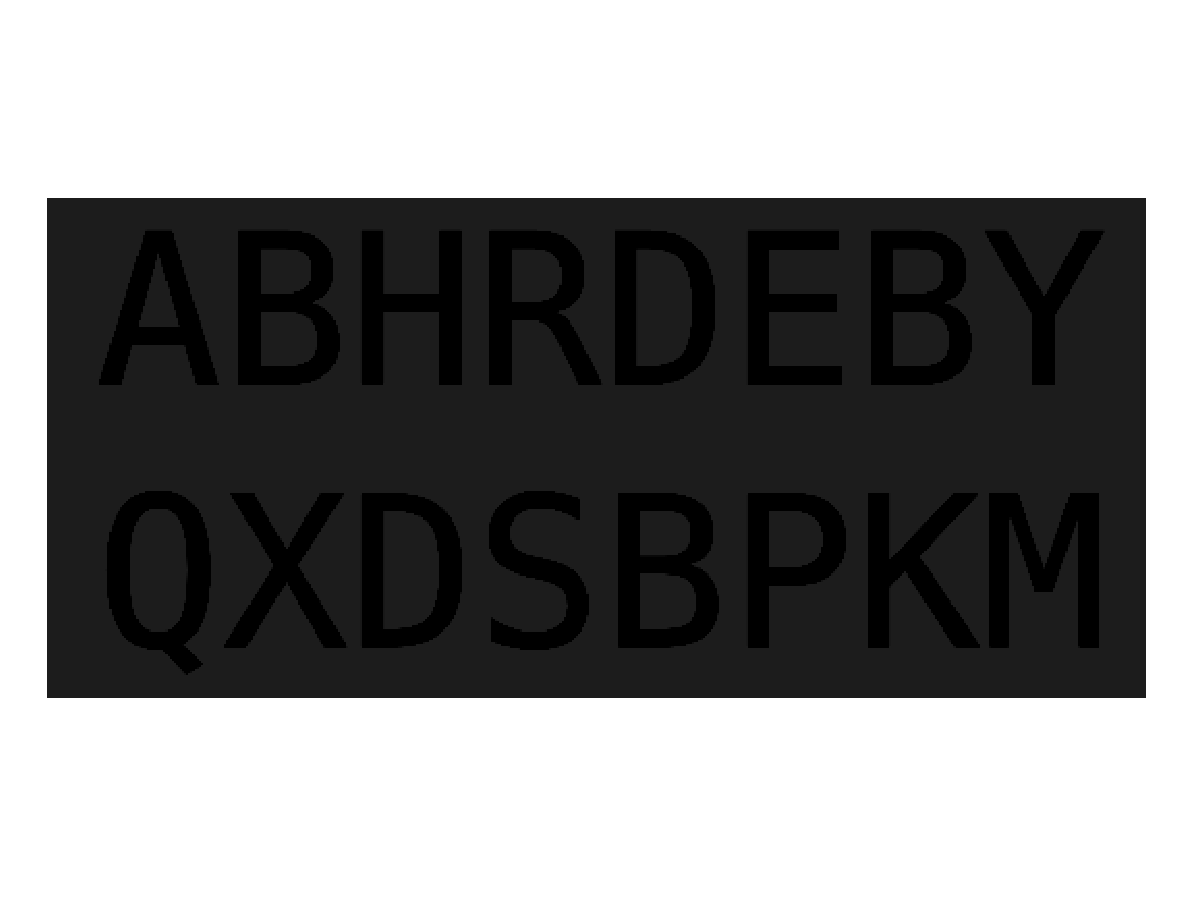
\includegraphics[scale=0.4]{../illus/motm0.png}\\
				Motif en niveaux de gris  & Image en niveaux de gris \\
				avec valeur moyenne nulle & avec valeur moyenne nulle\\
		\end{tabular}	
		\end{center}
		
		\subsubsection{La recherche}
		Maintenant que nos images sont prêtes on peut commencer à chercher le motif dans l'image. Pour cela nous allons utiliser l'intercorrélation. En calculant les coefficients de corrélation entre les deux images, on va pouvoir localiser où le motif original a été translaté horizontalement ou verticalement.
		Sur \octave nous utilisons la fonction \texttt{normxcorr2} afin d'obtenir les coefficients de corrélation normalisés. Cette fonction renvoie une matrice, d'une taille supérieure à l'image, contenant les coefficients d'intercorrélation. Plus le coefficient est proche de 1, plus le motif est semblable à la partie de l'image analysée.
		Nous pouvons représenter cette matrice sur un graphe et ainsi repérer les points de similitude.
		
		\begin{center}
			\begin{tabular}{cc}
				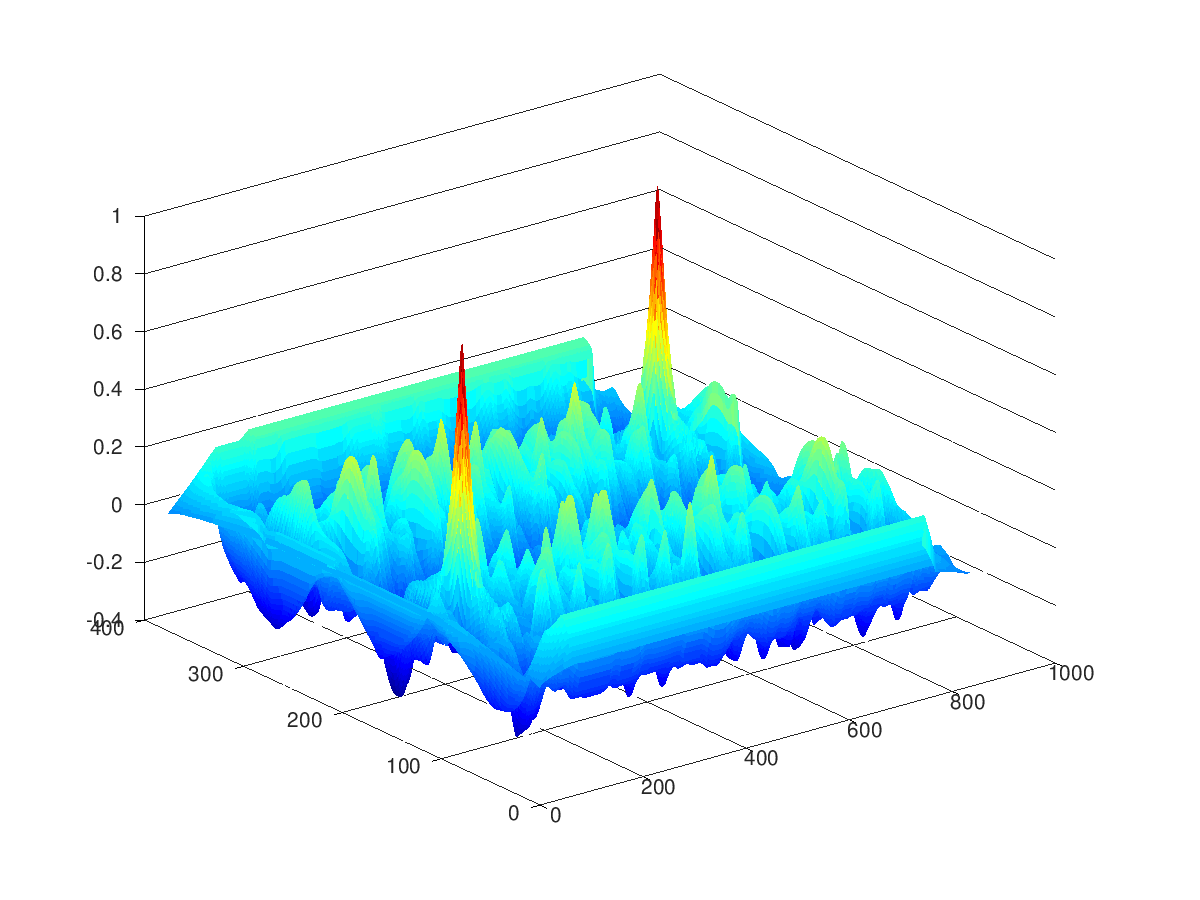
\includegraphics[scale=0.19]{../illus/cor.png} & 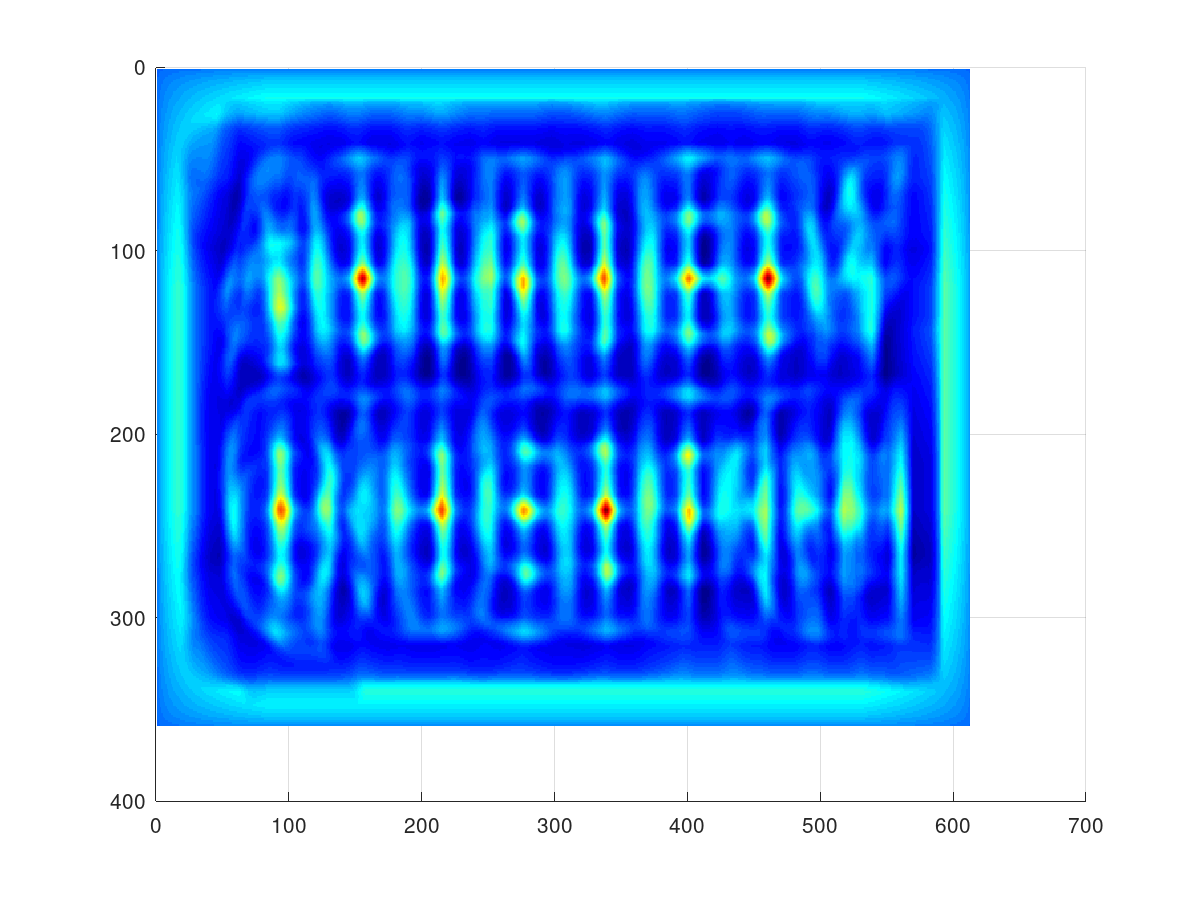
\includegraphics[scale=0.19]{../illus/cor1.png}\\
				Représentation des coefficients en 3D  & Représentation des coefficients vue de dessous\\
			\end{tabular}
		\end{center}
		
		Avec ces représentations, nous pouvons repérer les occurrences du motif dans l'image. Il faut maintenant récupérer les coordonnées des pics les plus hauts pour localiser le motif.
		\subsubsection{L'affichage}
		Dans la première partie de réalisation de ce projet, nous avons choisi de localiser les caractères recherchés et de représenter cette localisation. Nous avons donc décidé de dessiner un cercle autour des motifs repérés dans l'image.
		Ainsi après l'exécution du script, le dernier graphique affiché correspond à l'image en niveau de gris où des cercles sont tracés afin d'indiquer les points de similitude entre l'image et le motif.
		Afin de placer les cercles, nous parcourons la matrice de corrélation et nous récupérons les coordonnées de chaque point supérieur à un seuil donné. 

		\subsubsection{Problèmes restants}
		Après différents essais, nous pouvons montrer que certains problèmes persistent et seront à traiter par la suite.
		En effet, si la matrice représentant le motif à chercher n'est pas de la même taille que le motif dans l'image, la corrélation ne trouvera aucune correspondance. Pour résoudre ce problème, il faudra identifier la taille d'un caractère présent dans l'image pour faire correspondre la taille du motif.
		Avec notre technique actuelle, plusieurs points se situent au dessus de notre seuil, c'est pour cela que plusieurs cercles sont tracés pour chaque caractère reconnu. Résoudre ce problème se résumerait à identifier les points proches pour les "rassembler" en une seul occurrence du caractère.
	\subsection{Second essai}
	Après avoir essayer de corriger les problèmes développé ci-dessus, nous avons décider d'effectuer des changements dans l’algorithme de fonctionnement de base de notre script. Au lieu de travailler sur toute l'image, on découpe l'image en tuile contenant chacune un caractère, ainsi on applique la corrélation entre le motif et la tuile pour déterminer le caractère contenu dans la tuile.
	
\includegraphics[scale=0.5]{../illus/tuile.png}
	On se fait ensuite défiler nos motifs au dessus de chaque tuile pour trouver la meilleur correspondance.
	Le travail à effectuer se décompose en plusieurs étapes:
		\begin{itemize}
			\item[$\bullet$] charger et mettre en forme les images ;
			\item[$\bullet$] déterminer la taille des tuiles et le nombre de celle ci
			\item[$\bullet$] détecter le caractère présent
		\end{itemize}
	\subsubsection{L'image}
	Pour ce second essai, nous avons gardé les mêmes sources d'images que lors du premier essais en les modifiant légèrement (changement de tailles et de couleurs). Nous appliquons ensuite le même protocole de mise en forme, passage en niveau de gris, retrait de la valeur moyenne, etc...
	\subsubsection{Détermination de la taille des tuiles}
	Plusieurs méthodes étaient possible pour déterminer la taille des tuiles, nous avons dans un premier temps utilisé la taille des motifs pour déterminer la taille des caractères sur l'image à décoder, cette méthode est très performante mais ne permet pas de gérer des caractères de taille différente, en effet les valeurs sont liées dans le processus. Nous nous sommes donc basé sur les espaces inter-caractère. En effet entre chaque caractère un petit espace est présent, la police étant une police monospace, la taille des caractères est identiques et ils sont donc tous alignés sur une "grille". Cette espace est détectable, en effet en faisant la moyenne des valeurs la colonne on peut identifier les écarts.
	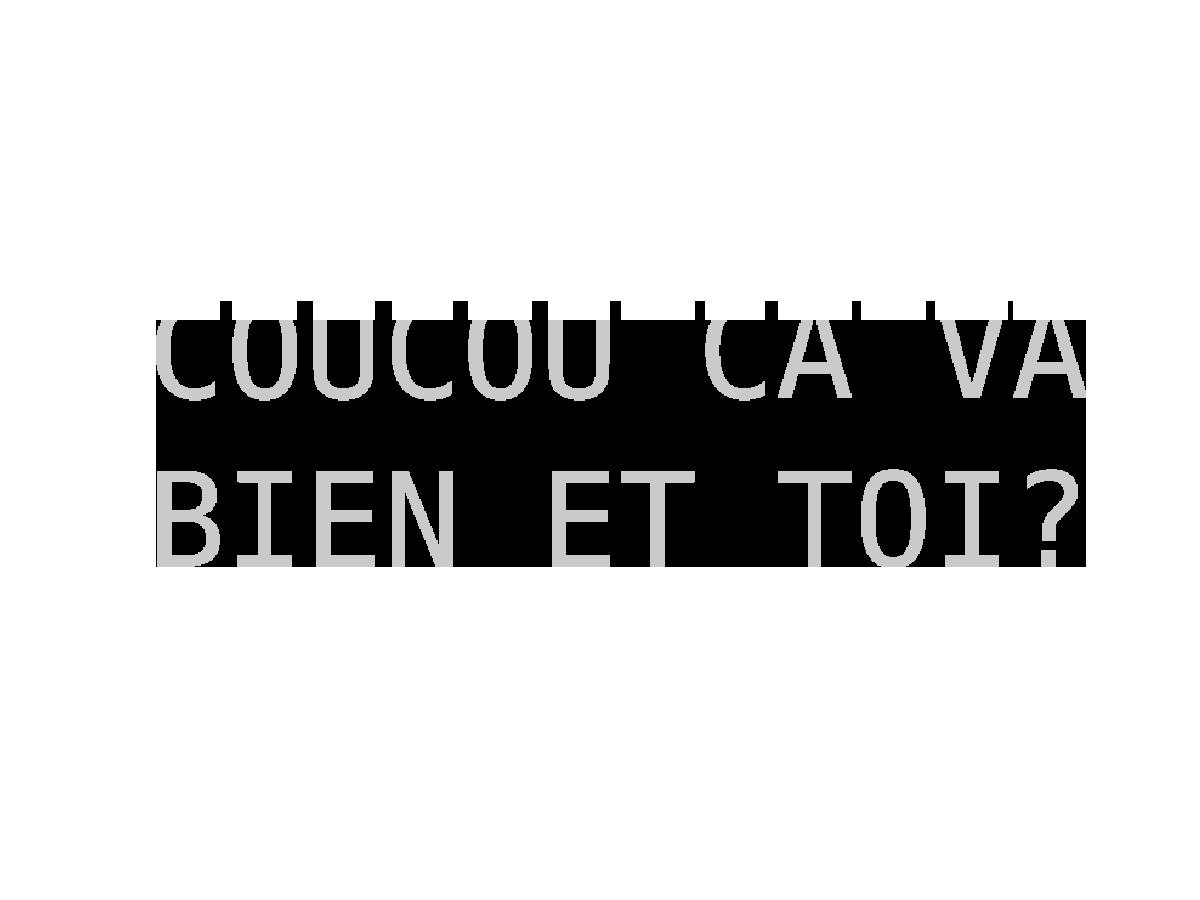
\includegraphics[scale=0.5]{../illus/detectionSpace.png}
	Ainsi en comptant le nombre d'espaces détecter nous pouvons déterminer le nombre de caractères par ligne.
	On effectue le même processus, en faisant la moyenne sur les lignes pour détecter le nombre de ligne.
	Il faut ensuite faire attention aux faux écarts, induit par les point et accents sur les lignes et par les espaces sur les colonnes.
	\subsubsection{Détermination du caractère}
	\subsubsection{Améliorations apportés au script de base}
	Nous avons commencé par écrire le script réalisant les fonctions basiques, nous avons ensuite ajouter différentes fonctionnalités pour améliorer notre script.
	\paragraph{Rapidité}
	Une fois l'algorithme de détection de caractères suffisamment robuste sur plusieurs exemples d'images, nous avons réfléchi à de nouvelles stratégies afin d'améliorer le temps de détection sur une image complète.
	\subparagraph{Arrêt de recherche corrélative sur prédiction de maximum}
	Explication du break
	\subparagraph{Recherche corrélative suivant un rangement des fréquences d'occurences de caractères}	 
	 Une des premières pistes a été de considérer l'aspect linguistique d'occurences statistiques des caractères dans des textes de la langue française. Le but était alors de tester la corrélation sur chaque tuile en considérant successivement les caractères du plus au moins répandu dans la langue française plutôt que l'ordre alphabétique traditionnel. Pour ce faire, une courte recherche bibliographique nous a amené sur le site web de typographie \textit{bépo} qui propose un \href{http://bepo.fr/wiki/Fr%C3%A9quence_des_caract%C3%A8res}{\textcolor{blue}{classement des occurences de caractères}} basé sur le corpus Wikipedia français de 2008. La \textsc{Table \ref{freq_carac}} 
\begin{table}
\begin{tabular}{|c|c|c|c|}
\hline
\textbf{Rang} & \textbf{Caractère} & \textbf{Nb d'occurrences} & \textbf{\%} \\
\hline
1 &	e &	115 024 205 & 12,1 \\
\hline
2 &	a &	67 563 628 & 7,11 \\
\hline
3 &	i &	62 672 992 & 6,59 \\
\hline
4 &	s &	61 882 785 & 6,51 \\
\hline
5 &	n &	60 728 196 & 6,39 \\
\hline
6 &	r &	57 656 209 & 6,07 \\
\hline
7 &	t &	56 267 109 & 5,92 \\
\hline
8 &	o &	47 724 400 & 5,02 \\
\hline
9 &	l &	47 171 247 & 4,96 \\
\hline
10 & u & 42 698 875 & 4,49 \\
\hline
11 & d & 34 914 685 & 3,67 \\
\hline
12 & c & 30 219 574 & 3,18 \\
\hline
13 & m & 24 894 034 & 2,62 \\
\hline
14 & p & 23 647 179 & 2,49 \\
\hline
15 & é & 18 451 937 & 1,94 \\
\hline
16 &   & 14 847 201 & 1,56 \\
\hline
17 & g & 11 684 140 & 1,23 \\
\hline
18 & b & 10 817 171 & 1,14 \\
\hline
19 & v & 10 590 858 & 1,11 \\ 
\hline
20 & h & 10 583 562 & 1,11 \\ 
\hline
21 & f & 10 579 192 & 1,11 \\
\hline
22 & , &  9 656 092 & 1,02 \\
\hline
23 & 1 &  9 005 786 & 0,95 \\
\hline
24 & . &  7 843 682 & 0,83 \\
\hline
25 & ' &  7 209 956 & 0,76 \\
\hline
26 & 0 &  6 358 672 & 0,67 \\
\hline
27 & 9 &  6 340 285 & 0,67 \\
\hline
28 & q &  6 140 307 & 0,65 \\
\hline
29 & - &  5 718 628 & 0,6  \\
\hline
30 & 2 &  5 462 613 & 0,57 \\
\hline
31 & y &  4 351 953 & 0,46 \\
\hline
32 & 8 &  3 643 296 & 0,38 \\
\hline
33 & ) &  3 638 248 & 0,38 \\
\hline
34 & ( &  3 624 542 & 0,38 \\
\hline
35 & x &  3 588 990 & 0,38 \\
\hline
36 & 3 &  3 459 061 & 0,36 \\
\hline
37 & 5 &  3 396 449 & 0,36 \\
\hline
38 & 6 &  3 376 188 & 0,36 \\
\hline
39 & 4 &  3 326 019 & 0,35 \\ 
\hline
40 & j &  3 276 064 & 0,34 \\
\hline
41 & 7 &  3 244 260 & 0,34 \\
\hline
42 & : &  3 155 250 & 0,33 \\
\hline
\end{tabular}
\begin{tabular}{|c|c|c|c|}
\hline
\textbf{Rang} & \textbf{Caractère} & \textbf{Nb d'occurrences} & \textbf{\%} \\
\hline
43 & è &  2 969 466 & 0,31 \\
\hline
44 & à &  2 966 029 & 0,31 \\
\hline
45 & k &  2 747 547 & 0,29 \\
\hline
46 & ? &  2 188 127 & 0,23 \\
\hline
47 & w &  1 653 435 & 0,17 \\
\hline
48 & z &  1 433 913 & 0,15 \\
\hline
49 & ê &	802 211 & 0,08 \\
\hline
50 & " &	759 384 & 0,08 \\
\hline
51 & / &	623 640 & 0,07 \\
\hline
52 & ç &	544 509 & 0,06 \\
\hline
53 & > &	499 481 & 0,05 \\
\hline
54 &\# &	493 596 & 0,05 \\
\hline
55 & < & 	476 762 & 0,05 \\
\hline
56 & · &	429 085 & 0,05 \\
\hline
57 &   &	402 911 & 0,04 \\
\hline
58 & ; &	379 874 & 0,04 \\
\hline
59 & ô &	357 197 & 0,04 \\
\hline
60 & « & 	338 547 & 0,04 \\
\hline
61 & » &	332 970 & 0,04 \\
\hline
62 & â &	320 837 & 0,03 \\
\hline
63 & î & 	280 201 & 0,03 \\
\hline
64 & ] &	243 399 & 0,03 \\
\hline
65 &\{ &	243 170 & 0,03 \\
\hline
66 & [ &	241 191 & 0,03 \\
\hline
67 &\} &	229 128 & 0,02 \\
\hline
68 &$^\circ$&214 463& 0,02 \\
\hline
69 & û &    164 516 & 0,02 \\
\hline
70 & ù &	151 236 & 0,02 \\
\hline
71 & ï &	138 221 & 0,01 \\
\hline
72 & = &	121 994 & 0,01 \\
\hline
73 &\% &	121 163 & 0,01 \\
\hline
74 & + &	109 254 & 0,01 \\
\hline
75 & ! &	104 109 & 0,01 \\
\hline
76 &\_ &	 87 702 & 0,01 \\
\hline
77 & á &	 73 751 & 0,01 \\
\hline
78 &\& &	 67 507 & 0,01 \\
\hline
79 & ü & 	 55 172 & 0,01 \\
\hline
80 &$^2$& 	 54 500 & 0,01 \\
\hline
81 & * &	 54 224 & 0,01 \\
\hline
82 & ë & 	 53 862 & 0,01 \\
\hline
83 & ö & 	 51 020 & 0,01 \\
\hline
84 & í &	 48 391 & 0,01 \\ 
\hline
\end{tabular}
\label{freq_carac}
\end{table}	

L'aspect intéressant de ce classement est notamment d'inclure les caractères spéciaux et de ponctuation que l'on trouve dans la plupart des textes. 

Afin d'implémenter la fréquence des caractères de la langue française , nous avons renommé les images.

\subparagraph{Détection des tuiles vides}
	
	\paragraph{Ponctuations et minuscules}
	\subsection{Améliorations futures et suites du projet}	
	\section{Conclusion}
	
\end{document}